%%%%Measurment methods for measuring/estimating energy consumption
\section{Measurement methods}
As the complexity and energy demand of today's electronics is developing rapidly it's  important to have a good model of the energy usage of in todays industry. Low-power design is therefore one of the biggest research topics in toady's electronics and has produces numerous methods for measuring or estimating the energy consumption of a device. There are several alternatives for modeling the energy consumption of a system where the main difference is that the energy either gets estimated or measured. The following section will present some of these methods. The quality of the estimation and measurement techniques varies from a 20\% error rate to as low as 0.1\%.  The energy consumption can either be estimated before the execution of the program as in software estimation, or it can be directly measured under execution as with a shunt resistor. The appropriate method to use depends on the system that is under measurement, as some of the methods require detailed knowledge of the system, while other threat the system as a black box.
\subsubsection{Shunt resistor}
A shunt resistor is often used to measure the energy consumption of a load because of its cost friendly and simple configuration \cite{Intersil} \cite{Infineon} \cite{Vishay}. The shunt is placed in series with the device and the power supply.

If the voltage drop $V_{shunt}$ is measured, the current I can be calculated by Ohms law:\begin{equation}
V_{shunt}=R_{shunt}*I
\end{equation}

$R_{shunt}$ should be of a small value so it doesn't interference with the circuit. The power used by the device can then be calculated by using the power relation \begin{equation}
P=V_{load}*I \\
\end{equation}
\begin{equation}
V_{load}= V_{supply}-V_{shunt}
\end{equation}
\newline The resistor value of the shunt should be of a small value to minimize the power dissipated by the shunt. In \cite{Intersil} it is explained how the resistance value, temperature coefficient and the temperature resistance of the shunt resistor will affect the accuracy of the measurement:
\begin{equation}
\Delta R= R_{initial}* \Delta T * T_{coefficient}\\
\label{rchange}
\end{equation}
\begin{equation}
 \Delta T = \theta * I^{2}*R_{sense}
\end{equation}

The temperature change in the shunt comes mainly from the heat of the power dissipation that is caused by the current flowing into it. A smaller package has a higher thermal resistance $\theta$ and therefore a higher resistance change when power dissipation increases. Figure \ref{fig:Powererror} from \cite{Intersil} shows the error of three different shunt resistors with different packages. 

\begin{minipage}[t]{0.8\textwidth}
\centering
    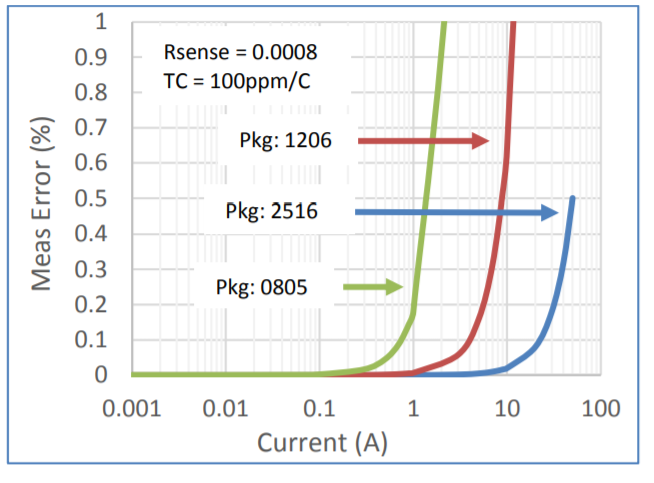
\includegraphics[width=0.8\textwidth]{Images/Powererror.PNG}\\
    \captionsetup{justification=centering}
    \captionof{figure}{The measurement error of three shunt resistors with different packages from \cite{Intersil}}
    \label{fig:Powererror}
\end{minipage}



\hfill \break
The shunt can be placed either in a high side or low side configuration. A low-side shunt has one of its terminals grounded, this configuration might be preferable as the shunt resistor is not exposed of the high common node voltage that might had damage the measurement device. The configuration does also give the measurement device an easy access to common ground so that more signals can be measured at the same time in reference to a stable ground. A high-side configuration places the shunt between the power supply and the load. This might be preferable because it connects the load directly to the ground of the power supply. This configuration enables the shunt to detect leakages that appear before the load, which may have not been detected by the low-side configuration. Figure \ref{fig:shunt} shows the two configurations. \hfill \break


\begin{figure}[h]
\centering
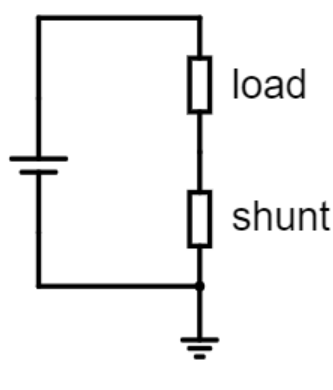
\includegraphics[height=4.5cm]{Project_Report/Images/shunt.PNG}
\caption{The setup for a low-side shunt and a high-side shunt to left and right respectively}
\label{fig:shunt}
\end{figure}







\subsection{Hall effect}
The Hall effect can be exploited to measure the current in the circuit. When a current $I$ flows in to a conductor it also changes the magnitude of the magnetic field $H$ proportionately. The relation between the flux density $B$ and $I$ can be expressed as follows:


\begin{equation}
B= \mu_{0}*\mu_{r}*H= \dfrac{\mu{0}*\mu{r}*I}{2\pi r}
\end{equation}

An Hall effect IC consists of a Hall effect sensor which deliver an output signal which is a linear function with the flux density. The IC is a a loss less system because no resistance is inserted into the circuit and therefore a good method of sensing current without interfering the load.  The IC does also require a field concentrator to boost the flux density for the measurement.
\begin{figure}[h]
\centering
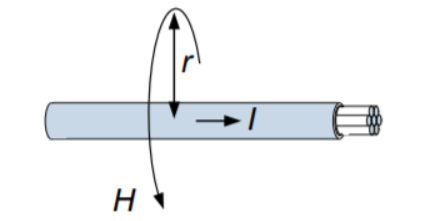
\includegraphics[height=4.5cm]{Project_Report/Images/current.PNG}
\caption{The induced magnetic field of a conductor from \cite{Infineon}}
\label{fig:current}
\end{figure}


\subsubsection{Software based estimation}

In \cite{EAC} Kadayif et al presents a framework that can estimate and optimize energy consumption of a high level code. The model is validated by using a cycle-accurate architectural-level energy simulator and is within a 6\% error margin.The input to the framework is its program code, architectural, transistor technology, energy model and the energy constraints.The paper uses a five staged pipeline datapath for the architectural parameter with a 0.35 micro transistor technology. The energy model that the framework uses is the sum of the energy consumed in different components. The components that are used to estimate the energy consumption consist of datapath, bus, main memory, cache and a clock network. Figure \ref{fig:EAC_table} shows the energy-dependent parameters of each component in the energy model and how they can be extracted from the high level code. The energy constraints are only used if optimization of the code is desired. 
\begin{figure}[H]
\centering
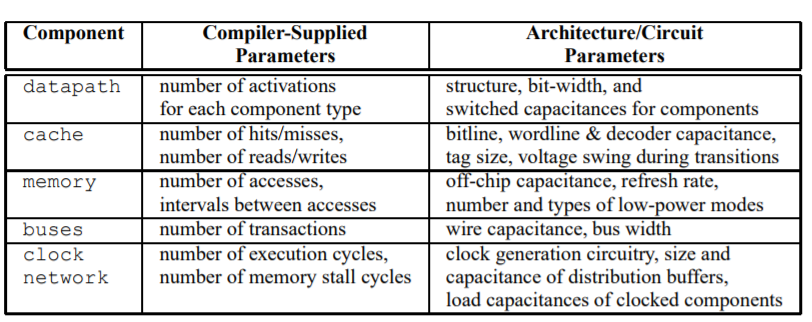
\includegraphics[height=4.5cm]{Project_Report/Images/EAC_table.PNG}
\caption{The energy dependent parameter of each component in the energy model and the belonging parameters in high-level code \cite{EAC}}
\label{fig:EAC_table}
\end{figure}
In \cite{Software_Energy} Deguang et al presents a method for estimating the energy consumption at architecture-level by using an extreme learning machine(ELM).  They model the architecture of the software system as a complex network, where the nodes are the software and the edges between them are the interactions. The energy model they proposed is given by \ref{software equation}

\begin{equation}
 E_{s}= P*T_{s} = f(m_{s})*T_{s}=f(V,E,L,K,C)*T_{s}
\label{software equation}
\end{equation}

$E_{s}$ is the total energy consumption over a $T_(s)$ period. P is the power consumption. $m_{s}$ is the network characteristics and f is the relation between the energy consumption and the network. f depends on the number of nodes V, the number of edges E, average path length L, the clustering coefficient L and the average degree of software network K. By using reverse software engineering they train the ELM to fit the nonlinear correlation function f and uses the ELM to estimate the energy consumption. They compare their model to a pTop model and achieves a 7.9\% error rate. 

\section{Cycle based energy estimation}
 Energy estimation can be done at RTL level by using cycle based energy models. In \cite{Energy_Gupta} Subdoh et al present a macro modeling technique for estimating the energy per cycle for a logic circuit for every input pair vector pair. The paper presents a automatically characterization procedure that can be used to build equation based energy per cycle macro models. The average error of the estimating the energy per cycle is under 20\%. \newline
 
 \cite{Energy_Ana} provides an approach for cycle-accurate hardware/software co-simulations of energy consumption. The simulation framework gets energy estimations for high level descriptions of embedded systems. The energy estimation is obtained by creating energy models for every hardware block and including them in functional models of the "Tool for system simulation"(TSS) simulator. An approach for creating energy models where no structural gate information is known is  presented in the article. 
 
 \cite{}